% !TEX root = ../Report.tex

tensorflow keras, (implement unet on our own, used library for DeepMedic)

graph loss on training evaluation (dice loss, bce dice loss, batch size (correlates to gpu), epochs, steps per epoch, optimizer)
prediction
image on label and prediction 
evaluating and examining models with hausdorff and mean distance on pictures (graphs or statistics, table)
comparison of unet and deepmedic

\begin{table}[h!]
	\centering
	\setlength{\tabcolsep}{10pt}
	\renewcommand{\arraystretch}{1.5}
	\begin{tabular}{c c c c}
		\hline 
		Architecture & Dice & Hausdorff & Mean \\ 
		& Coefficient & distance (mm) & Distance (mm) \\ 
		\hline 
		DeepMedic & 0.968 & 119.50 & 1.45 \\ 
		U-Net & 0.976 & 103.21 & 0.33 \\ 
		\hline 
	\end{tabular}
	\caption{Errors of the LSTM network compared to the forecasting approaches of assignment 1.}
	\label{table_result}
\end{table}


\begin{figure}[h!]
	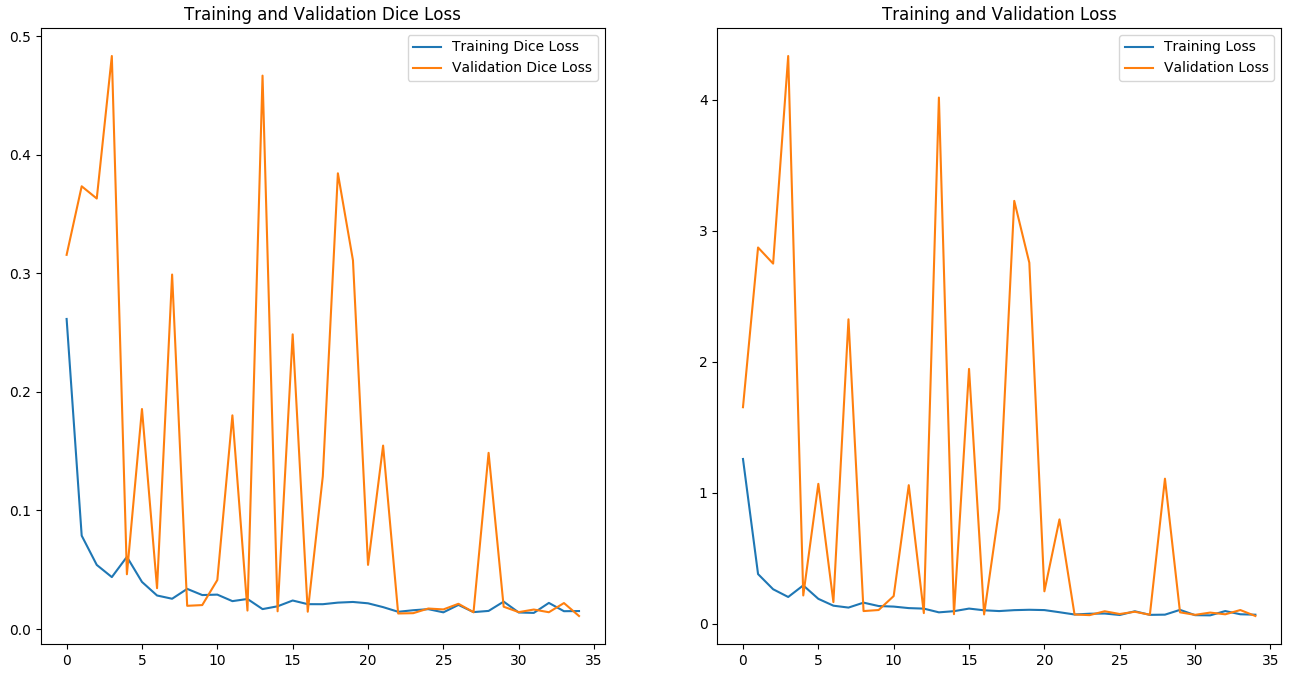
\includegraphics[width=0.49\textwidth, angle=0]{files/jpgunettrain.png}
	\caption{xxx}
	\label{scan_picture}
\end{figure}

\begin{figure}[h!]
	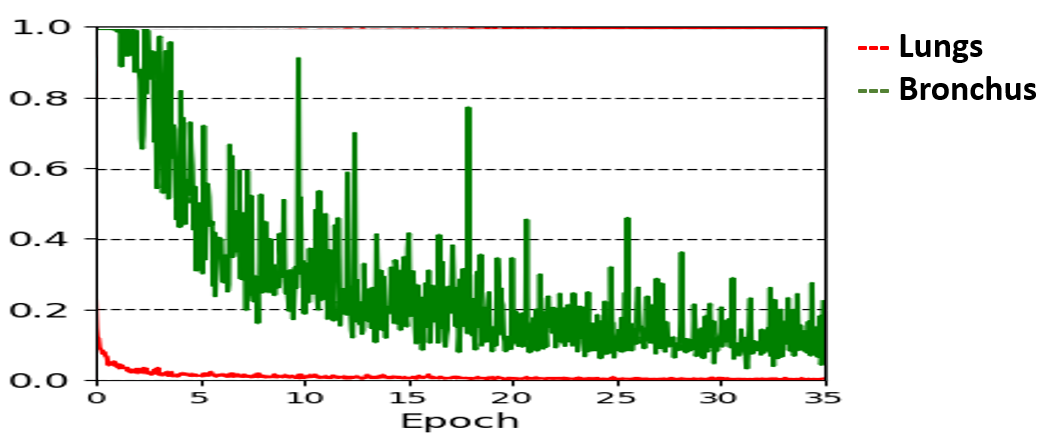
\includegraphics[width=0.49\textwidth, angle=0]{files/deepmedictrain.png}
	\caption{xxx}
	\label{scan_picture}
\end{figure}

\begin{figure}[h!]
	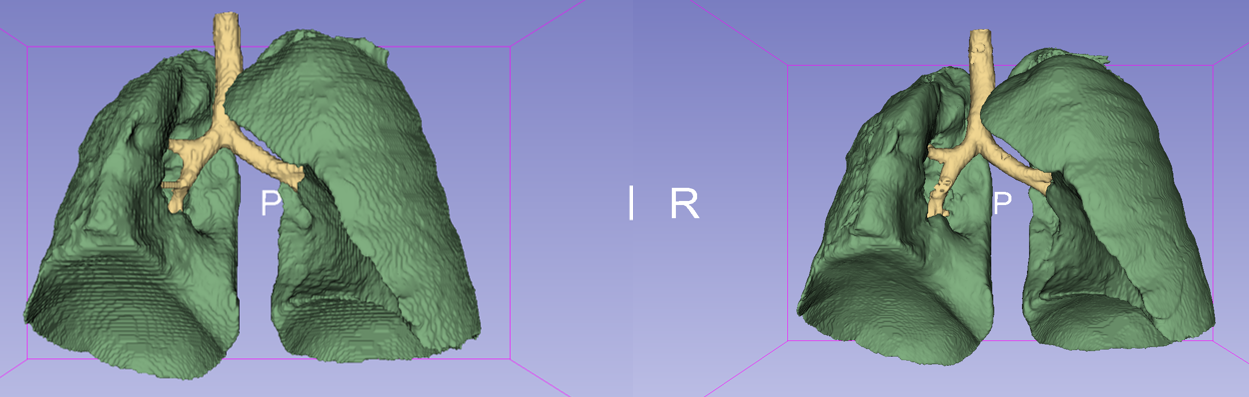
\includegraphics[width=0.49\textwidth, angle=0]{files/preddeepmedic.png}
	\caption{xxx}
	\label{scan_picture}
\end{figure}

\begin{figure}[h!]
	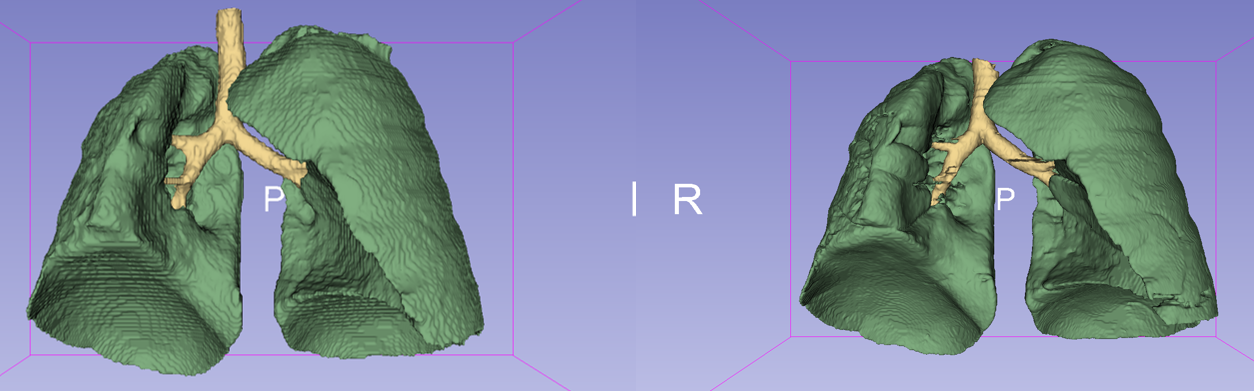
\includegraphics[width=0.49\textwidth, angle=0]{files/predunet.png}
	\caption{xxx}
	\label{scan_picture}
\end{figure}